% 要添加图片,左侧上传文件,然后这里输入 \figure 有自动提示回车,在回车地方加上图片名字
% 另起一段要换两行
% 表格在https://www.tablesgenerator.com/里复制
\begin{abstract}
    在现实世界中,有许多金融企业在运营中爆发危机的案例,例如1998年LTCM公司遭遇俄债违约导致巨额亏损、2008年雷曼兄弟破产。许多情况下人们将金融危机的爆发归结于企业风险管理的失败,但是\citeauthor{stulz2008risk}的这篇文章\citetitle{stulz2008risk}认为金融危机的爆发并不能说明企业的风险管理失败,作者定义了六种类型的风险管理失败,并结合LTCM的案例逐一进行分析。
\end{abstract}
\section{文献背景}
美国长期资本管理公司(Long-Term Capital Management,LTCM)是 1994 年在美国创立的一家对冲基金公司。这家公司有两位天才核心成员迈伦·斯克尔斯(Myron Scholes)和罗伯特·默顿(Robert Merton)。他们建立了决定期权价格的模型 Black-Scholes,简称B-S期权定价模型。LTCM自创立以来,一直保持骄人的业绩,在华尔街乃至全世界一路高歌。这个汇聚了职业巨星、公关巨星、学术巨星的精英团队在创立之后的 4 年里取得了辉煌的业绩,收益报酬率高达20\%,很多大型银行和富豪们争先恐后地把资金委托给LTCM 管理。

LTCM采取了配对套利交易策略,配对套利交易是利用性质相似的两个资产之间存在一定价格关系而进行的方向相反的交易活动,其中最负盛名也是最终导致LTCM坍塌的是债券利差交易,其交易标的包括全球各国的政府国债、公司债券以及房屋抵押证券等。第一步,通过公司内部及其复杂的数学模型计算出利差,预期两种债券间的利差在未来将会缩小;第二步,当期融券价格被高估的债券并卖出,然后买入价格被低估的债券;第三步,当未来两者的利差缩小时,多头空头同时获利。同时,为了进一步扩大收益,LTCM极度信任自己的数学模型,加了极高的杠杆进行套利交易,在1998年时,公司的杠杆率高达25倍。

通过如此激进的套利交易模式,从 1994 年 4 月开始运作到 1997 年 10 月,LTCM 累计投资回报率高达 300\%,公司的资产净值从成立之初的 10 亿美元上升到 47 亿美元。

在国际债券市场上,公司预期俄罗斯、日本等国家的债券价格被低估,未来这些国家与美国、德国等发达国家的政府债券利差将进一步缩小,因此LTCM持有俄罗斯、日本国债的多头,并利用美国国债的空头来对冲。

1998年8月17日,而当天俄罗斯政府突然宣布卢布贬值,并宣布冻结281亿卢布(135亿美元)的国债,停止国债交易。之后这一事件迅速发酵,致使诸多新兴市场的资信严重恶化,投资者纷纷从新兴市场撤出转而投向美国、德国风险更小、质量更高的债券品种。而此举直接导致的后果就是,西方国家与新兴市场的债券价差大幅拉开,LTCM由此遭受暴击。

到1998年8月底,LTCM的资本就已经降到了23亿美元,失去了年初时超过半数的股权资本。考虑到当时LTCM的资产基数约为1070亿美元,所以公司的杠杆比率已超过45倍。LTCM还开始遭受之前运营风格的“反噬”。由于LTCM对策略和持仓持有非常严格的保密协议,他们会将每个策略分割成不同的交易,分别交给不同的银行执行,使得别人无法猜到他们在做什么。这样的做法就使得在风险爆发之时,如果公司合约分属不同的交易对手,那么LTCM需要为每个交易对手都提供高昂的保证金。但是随着亏损的增加,当时的LTCM已经难以缴纳足够的保证金,甚至也缺少能够用来抵押的高价值资产。就这样,LTCM开始一步一步走向破产的结局。
\begin{figure}[H]
    \centering
    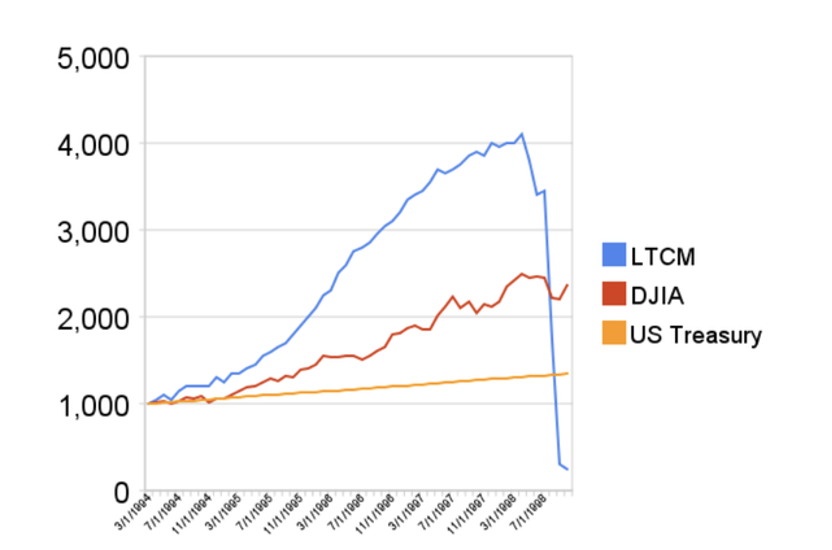
\includegraphics[width=\linewidth]{img/图片 1.png}
    \caption{LTCM基金净值走势与道琼斯指数及美国国债收益率对比}
\end{figure}
\section{风险管理失败的类型}
LTCM破产的案例中,使许多人将如此结果的原因归结于LTCM的风险管理失败,但是在文献中,作者认为LTCM遭遇俄债的可能只是正确管理风险后发生的极低概率损失事件。作者定义了六种风险管理的类型,分别为:
\begin{itemize}
    \item \nameref{sec:1}
    \item \nameref{sec:2}
    \item \nameref{sec:3}
    \item \nameref{sec:4}
    \item \nameref{sec:5}
    \item \nameref{sec:6}
\end{itemize}
\subsection{对已知风险的错误测量}\label{sec:1}
现实中,各家企业的风险管理部门依据数学模型、历史经验以及风险模拟来预测风险发生的概率分布,然后根据企业的风险容忍度做出相应的决策。如果企业对于风险发生的概率进行了错误的判断,例如将50\%可能发生的风险事件错误判断为只有10\%的概率发生,最终缺乏相应的风险控制导致了损失发生,那么这就是风险管理的失败。

以LTCM事件为例,公司内部的利差预测模型判断未来俄罗斯国债和美国国债利差将缩小,同时对于俄罗斯国债违约公司内部判断存在这样的风险会导致巨额损失,但是对于如此体量的国家来说出现违约属于极低概率事件,所以LTCM在识别出风险之后依然进行套利操作。

从这一角度判断,很难客观地权衡企业对于风险的预测是否正确,无法区分出究竟是预测的概率错误还是现实世界中确实发生了极小概率事件。我们认为, LTCM在对于俄罗斯政府的财务状况以及政府行为了解不充分,过度依赖于数学模型的预测结果,同期,有许多其他的公司正确预测了风险,认为俄罗斯有较大违约的可能性,已经提前撤出了在俄罗斯的资产。LTCM由于自身在风险预测上的不完备,低估了俄罗斯发生违约的概率,导致风险管理的失败。

\subsection{没有考虑到风险}\label{sec:2}
现实世界中存在各种各样的风险,因此企业的风险管理部门需要做好风险识别,如果遗漏了未知的风险,进行决策时没有考虑到,那么该风险一旦发生将会为企业带来巨大的损失。

该类型的风险管理失败一般后果极为严重,企业很难意识到。为了防止存在未识别的风险,需要事先进行仔细的调研分析。例如2021年的教育培训行业,许多私募基金投资人在投资该领域时,从未意识到延续了几十年的教培行业存在被政策叫停的风险,一般来说只会考虑投资教培行业的经营风险、财务风险等。当双减政策出台,许多叫教培企业一夜之间被迫关门,投资者面临了巨额的亏损。在LTCM的案例中,LTCM内部的风险报告中识别到了存在违约的可能性,因此从这一点来看,不属于是这一类型的风险管理失败。
\begin{figure}[H]
    \centering
    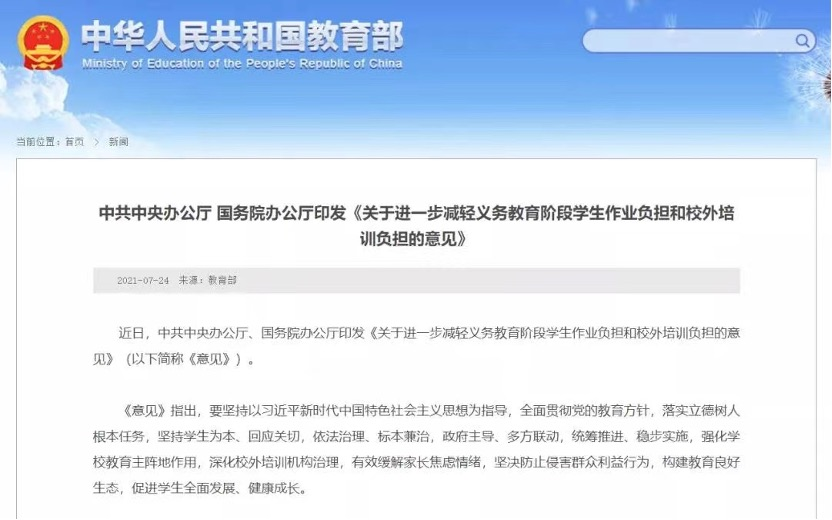
\includegraphics[width=\linewidth]{img/图片 1.jpg}
    \caption{2021年7月双减政策出台}
\end{figure}
\subsection{未能向最高管理层传达风险}\label{sec:3}
风险管理是为了使整个公司股东利益最大化而作出的行为,除了风险管理部门还需要各部门的协调配合,风险管理人员提供相关的风险信息,最终由管理层作出决策,各部门配合执行。但是如果企业内部的沟通失效,将会导致整个风险管理体系的失败。

内部沟通失败主要有两种情况,第一种是传递的信息出现扭曲,管理层错误理解了风险管理部门输出的信息,进而做出了不合适的决策;第二种是风险管理部门传递信息存在时滞,使风险管理体系失效。LTCM的例子中,我们认为并未出现沟通机制的失效,不存在这一类型的风险管理失败。
